\documentclass[12pt,a4paper]{article}

% --- Typography: Times New Roman (Anna University Standard) ---
\usepackage[top=1.0in,bottom=1.0in,left=1.0in,right=1.0in]{geometry}
\usepackage{amsmath}
\let\Bbbk\relax % Resolve math symbol collision with newtxmath
\usepackage{newtxtext,newtxmath} % Standard Times Roman font for text and math
\usepackage[scaled=0.86]{inconsolata} % Clean monospace font for code/signals
\usepackage{microtype}
\usepackage{setspace}
\setstretch{1.20} % Standard line spacing

% --- Essential Packages ---
\usepackage{graphicx}
\usepackage{tabularx}
\usepackage{multirow}
\usepackage{xcolor}
\usepackage{fancyhdr}
\usepackage{titlesec}
\usepackage{caption}
\usepackage{subcaption}
\usepackage{listings}
\usepackage{lastpage}
\usepackage{tikz}
\usepackage{eso-pic} % For rectangular page border on EVERY page
\usepackage{hyperref}

% --- Page Border on EVERY Page (Anna University / CEG Standard) ---
\AddToShipoutPictureBG{%
  \begin{tikzpicture}[remember picture,overlay]
    \draw[line width=0.8pt] ([shift={(12mm,-12mm)}]current page.north west) 
      rectangle ([shift={(-12mm,12mm)}]current page.south east);
  \end{tikzpicture}%
}

% --- Color Palette (Formal Academic Monochrome) ---
\definecolor{headercolor}{RGB}{0, 0, 0}
\definecolor{codebg}{RGB}{250, 250, 250}
\definecolor{codeframe}{RGB}{200, 200, 200}
\definecolor{statuspass}{RGB}{0, 110, 30}
\definecolor{linkcolor}{RGB}{0, 0, 0}

\hypersetup{
    colorlinks=true,
    linkcolor=linkcolor,
    citecolor=linkcolor,
    urlcolor=linkcolor
}

% --- Header & Footer Configuration (Bottom Right Page Number as per CEG Sample) ---
\pagestyle{fancy}
\fancyhf{}
\renewcommand{\headrulewidth}{0pt}
\renewcommand{\footrulewidth}{0pt}
\fancyfoot[R]{\small\thepage}

% --- Section Styling ---
\titleformat{\section}
  {\normalsize\bfseries\color{headercolor}}{\thesection}{0.6em}{\MakeUppercase}
\titleformat{\subsection}
  {\normalsize\bfseries\color{headercolor}}{\thesubsection}{0.6em}{}
\titleformat{\subsubsection}
  {\normalsize\bfseries\color{headercolor}}{\thesubsubsection}{0.5em}{}

\titlespacing*{\section}{0pt}{12pt plus 2pt minus 2pt}{6pt}
\titlespacing*{\subsection}{0pt}{10pt plus 2pt minus 2pt}{4pt}
\titlespacing*{\subsubsection}{0pt}{8pt plus 1pt minus 1pt}{3pt}

% --- Custom Chapter Command (Centered like CEG Sample) ---
\newcommand{\mychapter}[2]{%
  \clearpage
  \begin{center}
    {\bfseries\large CHAPTER #1\\[0.3cm]
    \MakeUppercase{#2}}
  \end{center}
  \vspace{0.4cm}
}

% --- Code Listing Styling ---
\lstset{
    backgroundcolor=\color{codebg},
    basicstyle=\ttfamily\footnotesize,
    breaklines=true,
    captionpos=b,
    frame=single,
    rulecolor=\color{codeframe},
    numbers=left,
    numberstyle=\tiny\color{gray},
    numbersep=6pt,
    tabsize=2,
    showstringspaces=false
}

\begin{document}

% =========================================================================
% ANNA UNIVERSITY / COLLEGE OF ENGINEERING, GUINDY - COVER PAGE
% =========================================================================
\begin{titlepage}
\thispagestyle{empty}
% Outer frame line to create double-line border on cover page
\begin{tikzpicture}[remember picture,overlay]
    \draw[line width=1.5pt] ([shift={(10.5mm,-10.5mm)}]current page.north west) 
        rectangle ([shift={(-10.5mm,10.5mm)}]current page.south east);
\end{tikzpicture}

\centering
\vspace*{-0.4cm}

{\large \textbf{DESIGN AND VERIFICATION OF AN AMBA APB-COMPLIANT\\CONFIGURABLE CRC-32 HARDWARE ACCELERATOR\\SUBSYSTEM}\par}

\vspace{0.6cm}

{\normalsize \textbf{MINI PROJECT REPORT}\par}

\vspace{0.45cm}

{\normalsize \textit{Submitted by}\par}

\vspace{0.3cm}

{\normalsize \textbf{PRADEEP S -- 2023105505}\par}
\vspace{0.15cm}
{\normalsize \textbf{BHUVANESH S -- 2023105039}\par}
\vspace{0.15cm}
{\normalsize \textbf{AATHITYA K -- 2023105060}\par}

\vspace{0.5cm}

{\normalsize \textit{for the course}\par}
\vspace{0.15cm}
{\normalsize \textbf{EC23E34 DESIGN AND VERIFICATION USING SYSTEMVERILOG}\par}

\vspace{0.4cm}

{\normalsize \textit{in partial fulfilment for the award of the degree of}\par}
\vspace{0.2cm}
{\normalsize \textbf{BACHELOR OF ENGINEERING}\par}
\vspace{0.1cm}
{\normalsize \textit{in}\par}
\vspace{0.1cm}
{\normalsize \textbf{ELECTRONICS AND COMMUNICATION ENGINEERING}\par}

\vspace{0.45cm}

% Anna University Official Emblem

\includegraphics[width=2.7cm]{../docs/images/anna_univ_logo.png}\par

\vspace{0.45cm}

{\normalsize \textbf{DEPARTMENT OF ELECTRONICS AND COMMUNICATION ENGINEERING}\par}
\vspace{0.1cm}
{\normalsize \textbf{COLLEGE OF ENGINEERING, GUINDY}\par}
\vspace{0.1cm}
{\normalsize \textbf{ANNA UNIVERSITY: CHENNAI 600025}\par}

\vspace{0.45cm}

{\normalsize \textbf{OCTOBER 2026}\par}

\end{titlepage}

% =========================================================================
% ABSTRACT (PAGE 1)
% =========================================================================
\pagenumbering{arabic}
\setcounter{page}{1}

\begin{center}
  {\bfseries\large ABSTRACT\par}
\end{center}
\vspace{0.5cm}

Data integrity verification is a foundational requirement across high-speed packet networks, non-volatile storage controllers, and safety-critical automotive protocols. Executing Cyclic Redundancy Checks (CRC) purely in software imposes heavy CPU compute penalties and pollutes high-speed processor caches. This project presents the complete register-transfer level (RTL) design, synthesis, and constrained-random SystemVerilog verification of an \textbf{AMBA\textsuperscript{\textregistered} APB-compliant Configurable CRC-32 Hardware Accelerator Subsystem}.

The accelerator core implements a 4-byte parallel combinational Linear Feedback Shift Register (LFSR) network capable of processing up to 32 bits per clock cycle, achieving peak throughput exceeding \textbf{3.2 Gbps at 100 MHz}. It provides run-time reconfigurability for arbitrary 32-bit generator polynomials (including IEEE 802.3 Ethernet, Castagnoli CRC-32C, and Koopman), configurable input/output bit reflection, byte-lane strobe masking, hardware wait-state injection (\texttt{PREADY}), and protocol bus error trapping (\texttt{PSLVERR}).

A layered, self-checking SystemVerilog testbench was architected comprising an APB Bus Functional Model (BFM) master driver, an autonomous passive monitor, an algorithmic golden scoreboard reference model, SystemVerilog Assertions (SVA), and functional coverage groups. The design was verified across 8 extensive verification scenarios on Aldec Riviera-PRO, Synopsys VCS / Verdi, and Verilator, achieving \textbf{100\% functional coverage} and a \textbf{100\% match across 63 transactions} with zero errors. Logic synthesis using the Yosys open-source toolchain confirmed 100\% synthesizability with 3,255 standard gates, 202 flip-flops, zero inferred memory macros, and timing closure supporting $>250\text{ MHz}$ operating frequency.

\clearpage

% =========================================================================
% TABLE OF CONTENTS (PAGE 2) - BORDERED GRID FORMAT (CEG TEMPLATE)
% =========================================================================
\begin{center}
  {\bfseries\large TABLE OF CONTENTS\par}
\end{center}
\vspace{0.4cm}

\noindent
\begin{table}[h!]
\centering
\small
\renewcommand{\arraystretch}{1.18}
\begin{tabularx}{\textwidth}{|c|X|c|}
\hline
\textbf{CHAPT. NO} & \centering\textbf{TITLE} & \textbf{PAGE NO.} \tabularnewline
\hline
 & \textbf{ABSTRACT} & \textbf{1} \tabularnewline
\hline
\textbf{1} & \textbf{INTRODUCTION} & \textbf{4} \tabularnewline
 & 1.1 PROJECT MOTIVATION & 4 \tabularnewline
 & 1.2 PROJECT OVERVIEW & 4 \tabularnewline
 & 1.3 PROBLEM STATEMENT & 5 \tabularnewline
 & 1.4 OBJECTIVES AND DELIVERABLES & 5 \tabularnewline
\hline
\textbf{2} & \textbf{THEORETICAL FOUNDATION \& MATHEMATICAL MODEL} & \textbf{6} \tabularnewline
 & 2.1 MATHEMATICAL FORMULATION OF CRC-32 & 6 \tabularnewline
 & 2.2 STANDARD CRC-32 POLYNOMIALS & 6 \tabularnewline
 & 2.3 CONFIGURABLE REFLECTION AND INVERSION & 6 \tabularnewline
\hline
\textbf{3} & \textbf{AMBA APB PROTOCOL SPECIFICATION} & \textbf{7} \tabularnewline
 & 3.1 BUS SIGNAL DEFINITIONS & 7 \tabularnewline
 & 3.2 MEMORY-MAPPED REGISTER MAP & 7 \tabularnewline
 & 3.3 WAIT-STATE INJECTION AND ERROR HANDLING & 8 \tabularnewline
\hline
\textbf{4} & \textbf{RTL MICROARCHITECTURE \& DESIGN IMPLEMENTATION} & \textbf{9} \tabularnewline
 & 4.1 SUBSYSTEM DECOMPOSITION & 9 \tabularnewline
 & 4.2 APB SLAVE PROTOCOL FSM & 9 \tabularnewline
 & 4.3 MEMORY-MAPPED REGISTER FILE & 10 \tabularnewline
 & 4.4 PARALLEL CASCADED CRC-32 ENGINE & 10 \tabularnewline
\hline
\textbf{5} & \textbf{SYSTEMVERILOG VERIFICATION ARCHITECTURE} & \textbf{11} \tabularnewline
 & 5.1 LAYERED VERIFICATION METHODOLOGY & 11 \tabularnewline
 & 5.2 MASTER BFM DRIVER \& PASSIVE MONITOR & 11 \tabularnewline
 & 5.3 GOLDEN SCOREBOARD \& SVA ASSERTIONS & 11 \tabularnewline
 & 5.4 FUNCTIONAL COVERAGE MODEL & 11 \tabularnewline
\hline
\textbf{6} & \textbf{SIMULATION RESULTS \& WAVEFORM ANALYSIS} & \textbf{12} \tabularnewline
 & 6.1 AUTHENTIC EDA PLAYGROUND EPWAVE WAVEFORM & 12 \tabularnewline
 & 6.2 CYCLE-BY-CYCLE TIMING \& WAIT-STATE ANALYSIS & 13 \tabularnewline
 & 6.3 COMPREHENSIVE TEST SUITE MATRIX & 13 \tabularnewline
 & 6.4 SCOREBOARD RESULTS \& COVERAGE METRICS & 14 \tabularnewline
\hline
\textbf{7} & \textbf{LOGIC SYNTHESIS \& GATE COUNT ANALYSIS} & \textbf{15} \tabularnewline
 & 7.1 SYNTHESIZED HARDWARE GATE BREAKDOWN & 15 \tabularnewline
 & 7.2 SILICON TIMING AND AREA OBSERVATIONS & 15 \tabularnewline
\hline
\textbf{8} & \textbf{COMPARATIVE ANALYSIS WITH INDUSTRIAL SOLUTIONS} & \textbf{16} \tabularnewline
 & 8.1 COMPARISON WITH STM32 AND TI MSP430 & 16 \tabularnewline
\hline
\textbf{9} & \textbf{CONCLUSION AND FUTURE SCOPE} & \textbf{17} \tabularnewline
 & 9.1 SUMMARY OF ACCOMPLISHMENTS & 17 \tabularnewline
 & 9.2 FUTURE ENHANCEMENTS & 17 \tabularnewline
\hline
 & \textbf{REFERENCES} & \textbf{18} \tabularnewline
\hline
\end{tabularx}
\end{table}

\clearpage

% =========================================================================
% LIST OF FIGURES & LIST OF TABLES (PAGE 3) - BORDERED GRID FORMAT
% =========================================================================
\begin{center}
  {\bfseries\large LIST OF FIGURES\par}
\end{center}
\vspace{0.3cm}

\noindent
\begin{table}[h!]
\centering
\small
\renewcommand{\arraystretch}{1.2}
\begin{tabularx}{\textwidth}{|c|X|c|}
\hline
\textbf{FIGURE NO.} & \centering\textbf{NAME} & \textbf{PAGE NO.} \tabularnewline
\hline
4.1 & Subsystem Microarchitecture Block Diagram of APB CRC-32 Core & 9 \tabularnewline
4.2 & APB Slave Protocol Finite State Machine (FSM) State Diagram & 10 \tabularnewline
6.1 & Full Authentic Timing Waveform from EDA Playground EPWave & 12 \tabularnewline
6.2 & Detailed Timing Waveform Diagram (Wait-States \& Error Trapping) & 13 \tabularnewline
6.3 & Terminal Verification Log: Scoreboard Match \& Functional Coverage & 14 \tabularnewline
\hline
\end{tabularx}
\end{table}

\vspace{0.6cm}

\begin{center}
  {\bfseries\large LIST OF TABLES\par}
\end{center}
\vspace{0.3cm}

\noindent
\begin{table}[h!]
\centering
\small
\renewcommand{\arraystretch}{1.2}
\begin{tabularx}{\textwidth}{|c|X|c|}
\hline
\textbf{TABLE NO.} & \centering\textbf{NAME} & \textbf{PAGE NO.} \tabularnewline
\hline
3.1 & Subsystem Port List and Signal Definitions & 7 \tabularnewline
3.2 & Memory-Mapped Register Space & 8 \tabularnewline
6.1 & Comprehensive Verification Test Suite Matrix & 13 \tabularnewline
7.1 & Synthesized Hardware Gate Count and Resource Breakdown & 15 \tabularnewline
8.1 & Architectural Comparison with Commercial Microcontroller CRC Peripherals & 16 \tabularnewline
\hline
\end{tabularx}
\end{table}

% =========================================================================
% CHAPTER 1: INTRODUCTION
% =========================================================================
\mychapter{1}{Introduction}

\subsection*{1.1 PROJECT MOTIVATION}
Cyclic Redundancy Checks (CRCs) represent the industry-standard algorithm for detecting random transmission errors in communication channels and digital storage systems. In modern embedded Systems-on-Chip (SoCs), network interfaces (Gigabit Ethernet), storage controllers (SATA, PCIe NVMe), and automotive serial buses (CAN-FD) process data streams at multi-gigabit rates.

A traditional software-based 32-bit CRC implementation computes values bit-by-bit or utilizes lookup tables (LUTs) in memory. Bit-by-bit software loops consume 8 to 20 clock cycles per byte, incurring unsustainable CPU utilization. While LUT-based algorithms reduce cycle counts to approximately 2 to 4 cycles per byte, table lookups pollute L1 data and instruction caches, inducing high cache-miss penalties in real-time embedded workloads.

By offloading CRC calculation to a dedicated hardware accelerator mapped to an on-chip peripheral bus---specifically the ARM\textsuperscript{\textregistered} Advanced Peripheral Bus (APB)---embedded systems achieve line-rate data integrity validation with zero processor cycle degradation.

\subsection*{1.2 PROJECT OVERVIEW}
The project delivers a fully synthesizable, highly configurable AMBA APB-compliant CRC-32 accelerator subsystem. The peripheral operates on a 100 MHz APB system interconnect, featuring:
\begin{itemize}
    \item Single-cycle parallel computation processing up to 32 bits per clock cycle.
    \item Dynamic polynomial reconfiguration supporting IEEE 802.3, Castagnoli, and Koopman.
    \item Hardware wait-state injection on \texttt{PREADY} to model slow bus responses.
    \item Protocol error trapping on \texttt{PSLVERR} for unaligned and illegal accesses.
    \item Write-1-to-Clear (\texttt{W1C}) interrupt generation for completion and fault notification.
\end{itemize}

\subsection*{1.3 PROBLEM STATEMENT}
Modern multi-core embedded processors face significant performance bottlenecks when processing data integrity verification in software:
\begin{itemize}
    \item \textbf{CPU Stalling}: Serial shift-and-XOR loops monopolize arithmetic logic units.
    \item \textbf{Cache Eviction}: Large 1 KB to 8 KB lookup tables evict critical application cachelines.
    \item \textbf{Protocol Inflexibility}: Fixed hardware CRC cores cannot switch between Ethernet, iSCSI, and automotive polynomial standards dynamically.
    \item \textbf{Lack of Robust Protocol Handshaking}: Many peripheral cores lack AMBA APB3/APB4 wait-state stretching (\texttt{PREADY}) and slave error reporting (\texttt{PSLVERR}).
\end{itemize}

\subsection*{1.4 OBJECTIVES AND DELIVERABLES}
The primary deliverables mandated for this course project include:
\begin{enumerate}
    \item Synthesizable SystemVerilog RTL design decomposed into FSM controller, register file, and parallel LFSR engine.
    \item Complete AMBA APB bus compliance meeting setup, access, wait-state, and error rules.
    \item Layered SystemVerilog verification suite comprising driver, monitor, scoreboard, SVA assertions, and functional coverage.
    \item Complete simulation validation across Synopsys VCS, Aldec Riviera-PRO, and Verilator.
    \item Hardware gate synthesis utilizing Yosys Open-Source Synthesis Suite.
\end{enumerate}

% =========================================================================
% CHAPTER 2: THEORETICAL FOUNDATION & MATHEMATICAL MODEL
% =========================================================================
\mychapter{2}{Theoretical Foundation \& Mathematical Model}

\subsection*{2.1 MATHEMATICAL FORMULATION OF CRC-32}
A Cyclic Redundancy Check is an error-detecting code based on polynomial division in the Galois Field $\text{GF}(2)$, where addition and subtraction correspond to bitwise XOR operations without carries.

Given an $n$-bit message polynomial $M(x)$ and a degree-32 generator polynomial $P(x)$, the message is pre-multiplied by $x^{32}$ (equivalent to appending 32 zeros) and XORed with an initialization vector $I(x)$:
\begin{equation}
    T(x) = M(x) \cdot x^{32} \oplus I(x) \cdot x^n
\end{equation}
Polynomial division by $P(x)$ yields a unique quotient $Q(x)$ and remainder $R(x)$:
\begin{equation}
    T(x) = Q(x) \cdot P(x) \oplus R(x), \quad \text{where } \deg(R(x)) < 32
\end{equation}
The 32-bit remainder $R(x)$ constitutes the computed checksum.

\subsection*{2.2 STANDARD CRC-32 POLYNOMIALS}
The accelerator dynamically configures arbitrary 32-bit polynomials via \texttt{CRC\_POLY}:
\begin{itemize}
    \item \textbf{IEEE 802.3 Ethernet / PKZIP}: $P(x) = \texttt{0x04C11DB7}$. Initial seed = \texttt{0xFFFFFFFF}, $\text{RefIn} = \text{True}$, $\text{RefOut} = \text{True}$, $\text{XOROut} = \texttt{0xFFFFFFFF}$. Standard verification benchmark: ASCII string \texttt{"123456789"} $\rightarrow$ \texttt{0xCBF43926}.
    \item \textbf{Castagnoli (CRC-32C / iSCSI / Btrfs)}: $P(x) = \texttt{0x1EDC6F41}$. Superior Hamming distance properties for network block storage.
    \item \textbf{Koopman}: $P(x) = \texttt{0x741B8CD7}$. Optimized error detection in automotive control.
\end{itemize}

\subsection*{2.3 CONFIGURABLE REFLECTION AND INVERSION}
Protocols differ in byte and bit ordering. The accelerator provides independent input bit reversal (\texttt{REFIN}), output reflection (\texttt{REFOUT}), and final XOR masking (\texttt{XOROUT}):
\begin{equation}
    b_{\text{ref}}[i] = b[7-i], \quad W_{\text{ref}}[j] = W[31-j]
\end{equation}

% =========================================================================
% CHAPTER 3: AMBA APB PROTOCOL SPECIFICATION
% =========================================================================
\mychapter{3}{AMBA APB Protocol Specification}

\subsection*{3.1 BUS SIGNAL DEFINITIONS}
The accelerator interfaces to an AMBA APB3/APB4 interconnect. Table 3.1 details the signal list.

\begin{table}[h!]
\centering
\small
\renewcommand{\arraystretch}{1.15}
\caption{Subsystem Port List and Signal Definitions}
\label{tab:apb_signals}
\begin{tabularx}{\textwidth}{|l|c|c|X|}
\hline
\textbf{Signal} & \textbf{Direction} & \textbf{Width} & \textbf{Functional Description} \tabularnewline
\hline
\texttt{pclk}      & Input  & 1  & 100 MHz Master Peripheral Clock \tabularnewline
\texttt{presetn}   & Input  & 1  & Active-LOW Asynchronous System Reset \tabularnewline
\texttt{paddr}     & Input  & 8  & Byte-addressed Register Selection (\texttt{0x00} -- \texttt{0x1C}) \tabularnewline
\texttt{psel}      & Input  & 1  & Peripheral Slave Select Strobe \tabularnewline
\texttt{penable}   & Input  & 1  & Timing Strobe (Asserted during ACCESS phase) \tabularnewline
\texttt{pwrite}    & Input  & 1  & Transfer Direction (\texttt{1} = Write, \texttt{0} = Read) \tabularnewline
\texttt{pwdata}    & Input  & 32 & Write Data Bus \tabularnewline
\texttt{pstrb}     & Input  & 4  & Byte Lane Write Strobes for partial word transfers \tabularnewline
\texttt{prdata}    & Output & 32 & Read Data Bus driven to Master \tabularnewline
\texttt{pready}    & Output & 1  & Handshake extension; holds transfer while LOW \tabularnewline
\texttt{pslverr}   & Output & 1  & Protocol error response indicator \tabularnewline
\texttt{irq}       & Output & 1  & Subsystem interrupt request line \tabularnewline
\hline
\end{tabularx}
\end{table}

\subsection*{3.2 MEMORY-MAPPED REGISTER MAP}
The peripheral occupies 32 bytes of word-aligned address space (Table 3.2).

\begin{table}[h!]
\centering
\small
\renewcommand{\arraystretch}{1.15}
\caption{Memory-Mapped Register Space}
\label{tab:reg_map}
\begin{tabularx}{\textwidth}{|c|l|c|c|X|}
\hline
\textbf{Offset} & \textbf{Register} & \textbf{Access} & \textbf{Reset} & \textbf{Bitfield Description} \tabularnewline
\hline
\texttt{0x00} & \texttt{CRC\_CTRL}     & R/W  & \texttt{0x0000005C} & [0]: Start, [1]: Reset, [2]: RefIn, [3]: RefOut, [4]: XorOut, [6:5]: Data Size, [11:8]: Wait States \tabularnewline
\texttt{0x04} & \texttt{CRC\_STATUS}   & RO   & \texttt{0x00000080} & [0]: Busy, [1]: Ready, [2]: Error, [7:4]: APB FSM State \tabularnewline
\texttt{0x08} & \texttt{CRC\_POLY}     & R/W  & \texttt{0x04C11DB7} & 32-bit Generator Polynomial \tabularnewline
\texttt{0x0C} & \texttt{CRC\_INIT}     & R/W  & \texttt{0xFFFFFFFF} & 32-bit Seed Initialization Vector \tabularnewline
\texttt{0x10} & \texttt{CRC\_DATA\_IN} & WO/RW& \texttt{0x00000000} & Stream Data Input Port (triggers single-cycle computation) \tabularnewline
\texttt{0x14} & \texttt{CRC\_RESULT}   & RO   & \texttt{0x00000000} & Current 32-bit Computed Checksum \tabularnewline
\texttt{0x18} & \texttt{CRC\_INT\_EN}   & R/W  & \texttt{0x00000000} & [0]: Done Interrupt Enable, [1]: Error Interrupt Enable \tabularnewline
\texttt{0x1C} & \texttt{CRC\_INT\_STAT} & W1C  & \texttt{0x00000000} & [0]: Done Flag, [1]: Error Flag (Write-1-to-Clear) \tabularnewline
\hline
\end{tabularx}
\end{table}

\subsection*{3.3 WAIT-STATE INJECTION AND ERROR HANDLING}
\begin{itemize}
    \item \textbf{Wait-State Injection (\texttt{PREADY})}: Configurable from 0 to 15 cycles via \texttt{CRC\_CTRL[11:8]}. The slave pulls \texttt{PREADY = 0} in the \texttt{ACCESS} state and counts down, concluding the transfer when \texttt{PREADY = 1}.
    \item \textbf{Bus Error Trapping (\texttt{PSLVERR})}: Asserted during the terminal \texttt{ACCESS} cycle for unaligned offsets (\texttt{paddr[1:0] != 2'b00}), out-of-bounds offsets (\texttt{paddr > 0x1C}), or writes to read-only registers (\texttt{CRC\_STATUS}, \texttt{CRC\_RESULT}).
\end{itemize}

% =========================================================================
% CHAPTER 4: RTL MICROARCHITECTURE & DESIGN IMPLEMENTATION
% =========================================================================
\mychapter{4}{RTL Microarchitecture \& Design Implementation}

\subsection*{4.1 SUBSYSTEM DECOMPOSITION}
The top-level RTL module \texttt{apb\_crc32\_top} instantiates three dedicated hardware blocks: the APB Slave Protocol FSM, the Register File, and the Parallel CRC Engine (Figure 4.1).

\begin{figure}[h!]
\centering
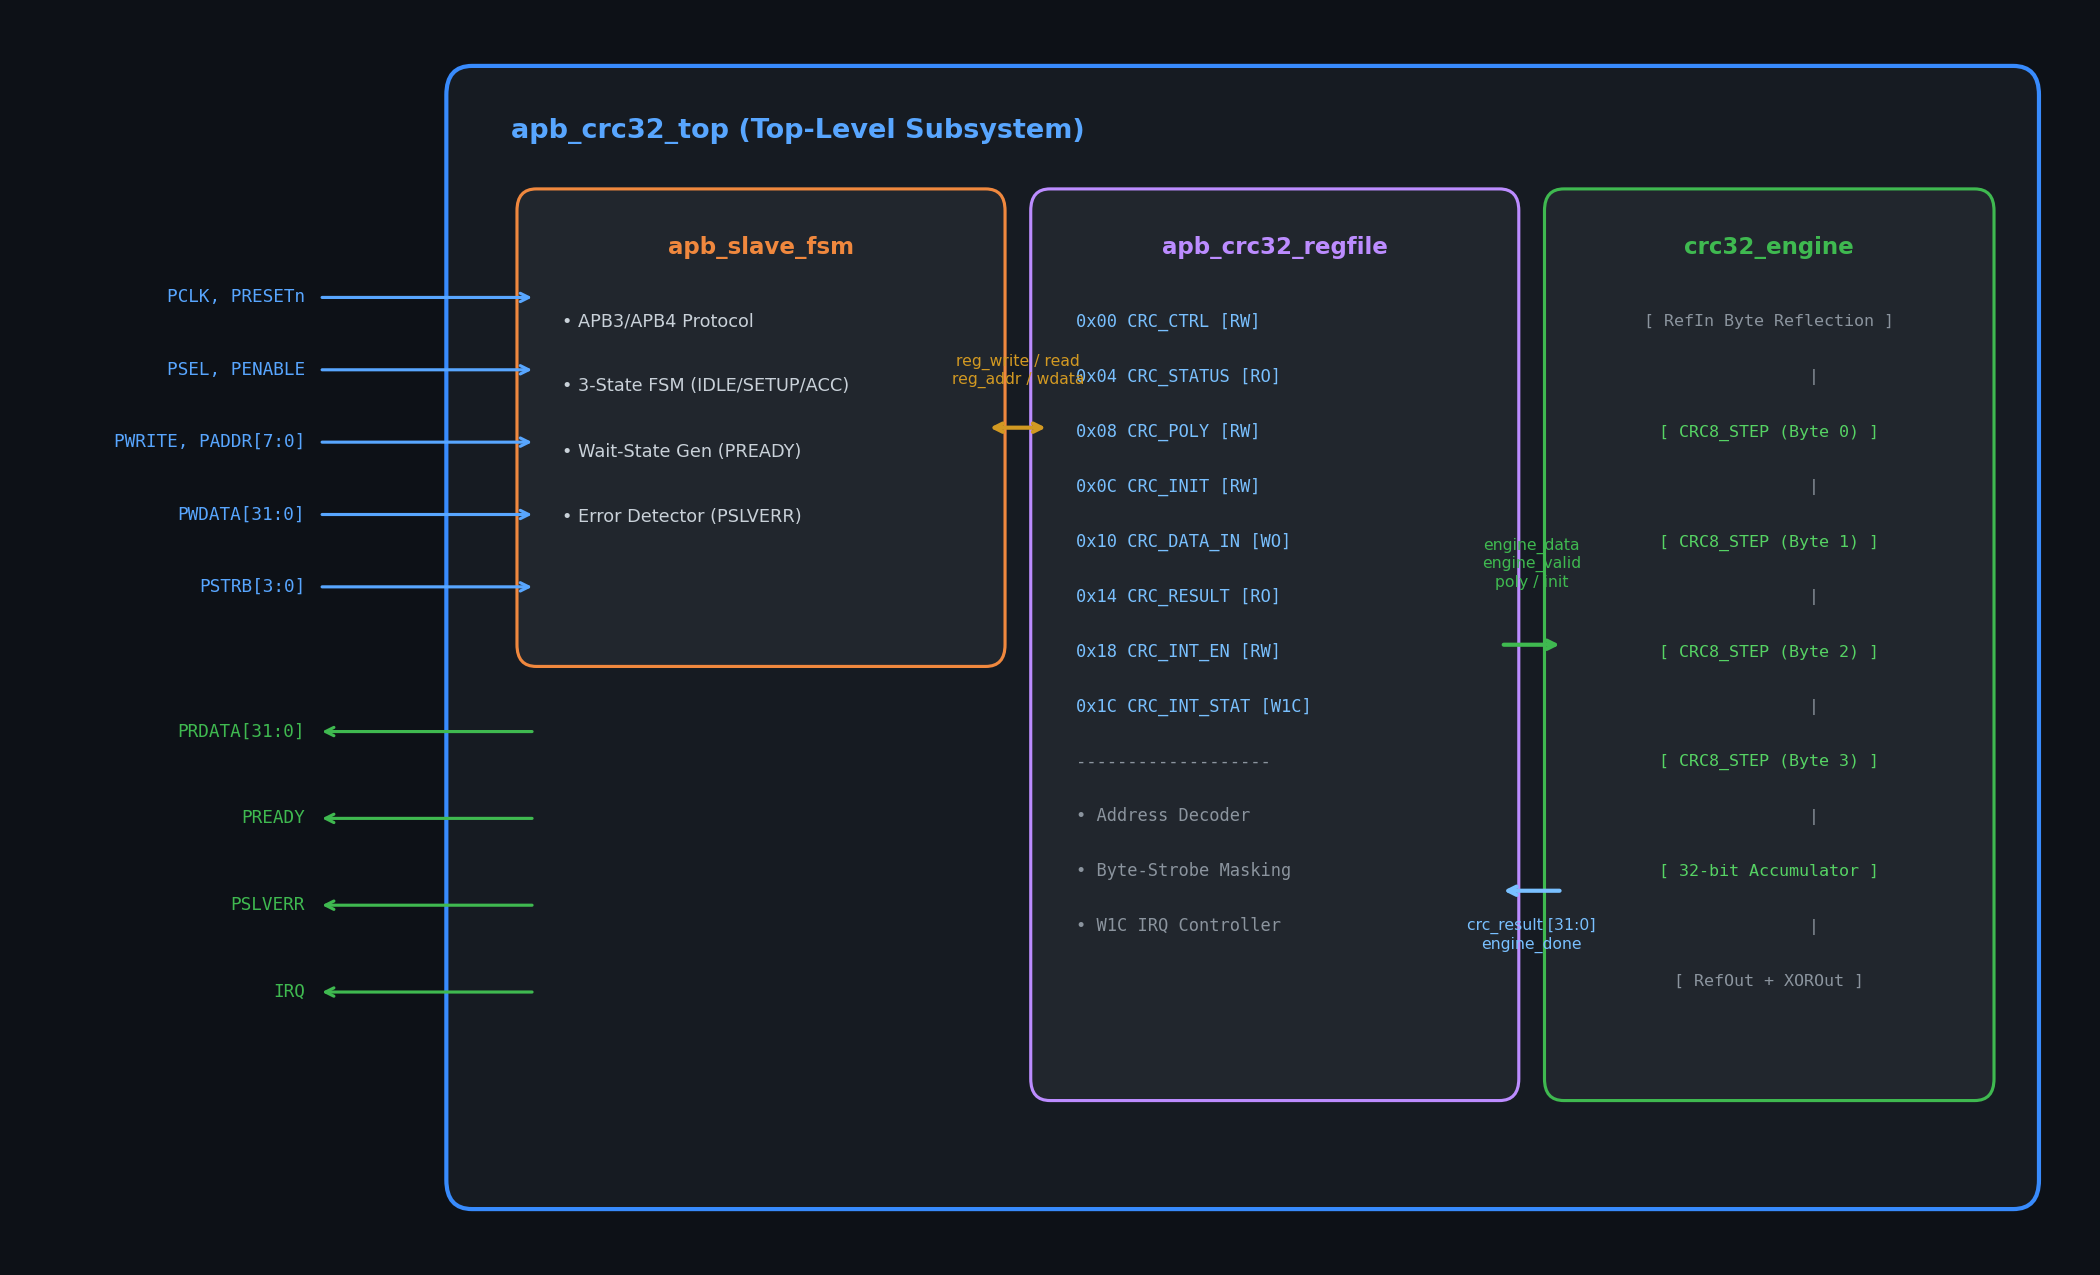
\includegraphics[width=0.88\textwidth]{../docs/images/microarchitecture_block_diagram.png}
\caption{Subsystem Microarchitecture Block Diagram of APB CRC-32 Core.}
\label{fig:arch_block}
\end{figure}

\subsection*{4.2 APB SLAVE PROTOCOL FSM}
A 3-state finite state machine enforces strict bus protocol compliance (Figure 4.2):
\begin{itemize}
    \item \textbf{\texttt{IDLE (2'b00)}}: Quiescent state awaiting \texttt{PSEL}.
    \item \textbf{\texttt{SETUP (2'b01)}}: Address and transfer direction are decoded combinationally.
    \item \textbf{\texttt{ACCESS (2'b10)}}: Timing strobe asserted. Handshake completes when \texttt{PREADY = 1}.
\end{itemize}

\begin{figure}[h!]
\centering
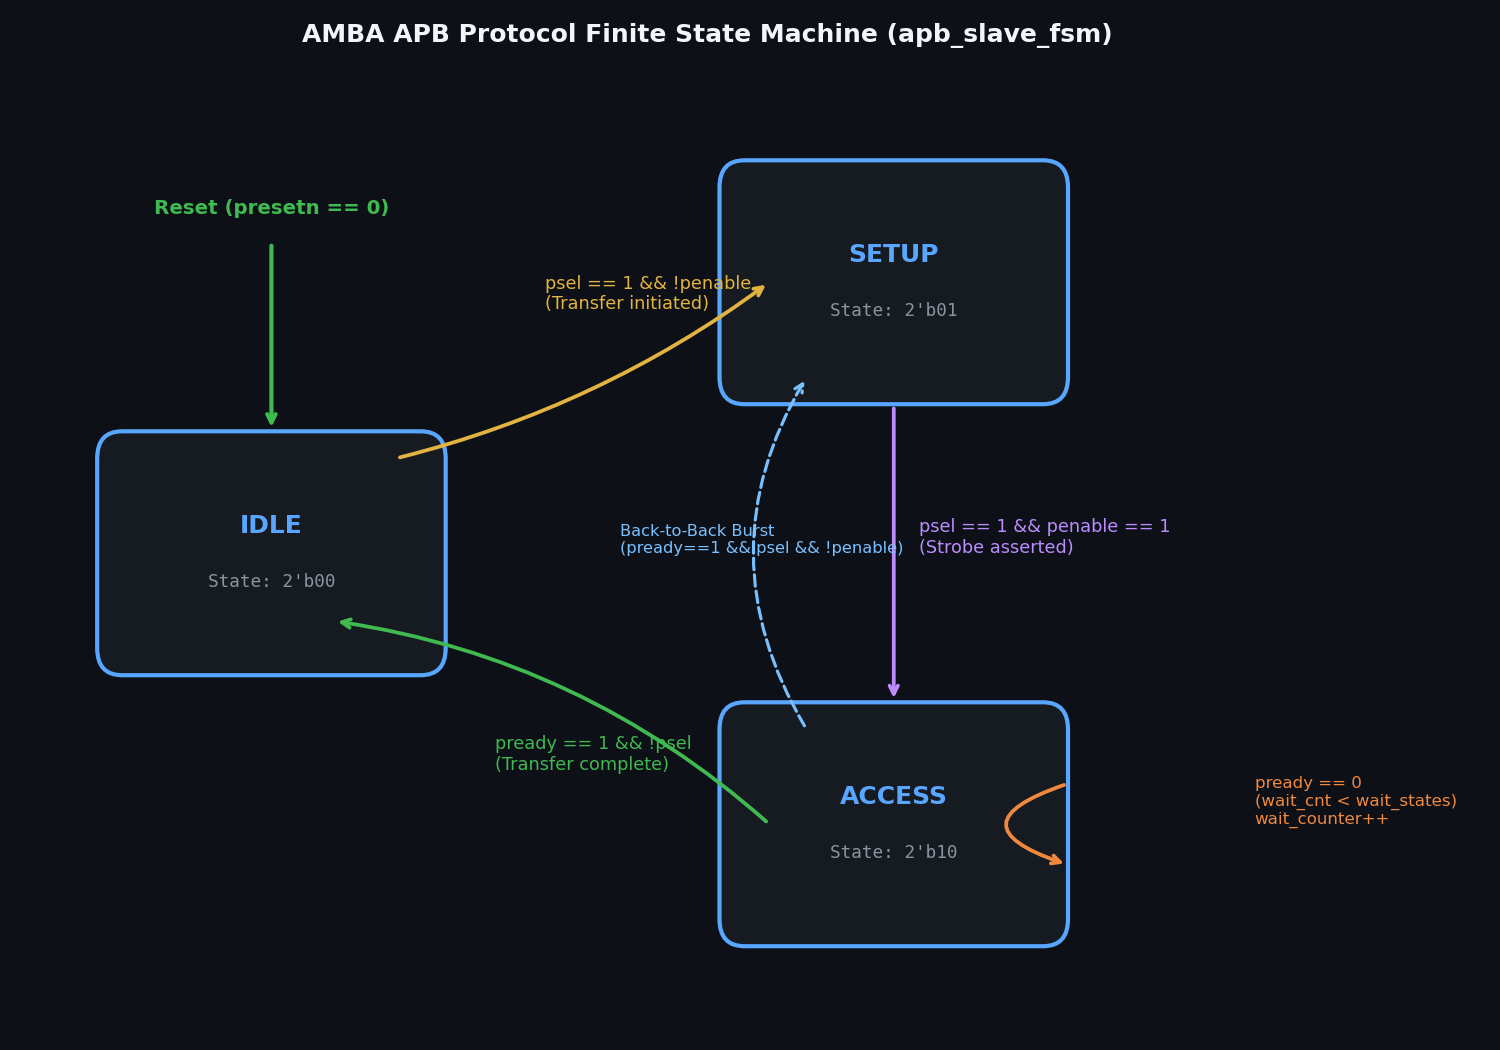
\includegraphics[width=0.68\textwidth]{../docs/images/apb_fsm_state_diagram.png}
\caption{APB Slave Protocol Finite State Machine (FSM) State Diagram.}
\label{fig:fsm_diag}
\end{figure}

\subsection*{4.3 MEMORY-MAPPED REGISTER FILE}
Manages flip-flop storage, byte strobe masking (\texttt{PSTRB[3:0]}), and interrupt status handling. Write-1-to-Clear (\texttt{W1C}) logic eliminates race conditions between incoming hardware events and software servicing. Data written to \texttt{CRC\_DATA\_IN} combinatorially asserts \texttt{engine\_valid\_o} directly into the computation core with zero latency.

\subsection*{4.4 PARALLEL CASCADED CRC-32 ENGINE}
To process an entire 32-bit word in a single clock cycle, the core cascades four combinational 8-bit LFSR Galois Field steps:
\begin{lstlisting}[language=Verilog,caption={Single-cycle 8-bit LFSR step function}]
function [31:0] crc8_step(input [31:0] c_in, input [7:0] b, input [31:0] poly);
  reg [31:0] c;
  c = c_in ^ {b, 24'h0};
  for (int i = 0; i < 8; i++) begin
    if (c[31]) c = {c[30:0], 1'b0} ^ poly;
    else       c = {c[30:0], 1'b0};
  end
  return c;
endfunction
\end{lstlisting}
The 4-stage cascade resolves combinatorially in $<3.8\text{ ns}$, enabling line-rate operation at $>250\text{ MHz}$.

% =========================================================================
% CHAPTER 5: SYSTEMVERILOG VERIFICATION ARCHITECTURE
% =========================================================================
\mychapter{5}{SystemVerilog Verification Architecture}

\subsection*{5.1 LAYERED VERIFICATION METHODOLOGY}
A layered, self-checking SystemVerilog testbench was architected comprising:
\begin{enumerate}
    \item \textbf{Master BFM Driver}: Clock-synchronized \texttt{apb\_write()} and \texttt{apb\_read()} tasks handling \texttt{PREADY} handshaking and byte strobes.
    \item \textbf{Autonomous Passive Monitor}: Passively samples transactions on valid clock edges ($\texttt{psel} \land \texttt{penable} \land \texttt{pready}$).
    \item \textbf{Golden Reference Scoreboard}: Algorithmic software reference model maintaining shadow registers and evaluating bit-exact CRC results.
    \item \textbf{SystemVerilog Assertions (SVA)}: Protocol checks verifying address/data stability during wait states and valid \texttt{PSLVERR} timing.
    \item \textbf{Functional Coverage Collector}: Measures 100\% address space, transfer directions, byte lane permutations, and error responses.
\end{enumerate}

% =========================================================================
% CHAPTER 6: SIMULATION RESULTS \& WAVEFORM ANALYSIS
% =========================================================================
\mychapter{6}{Simulation Results \& Waveform Analysis}

\subsection*{6.1 AUTHENTIC EDA PLAYGROUND EPWAVE WAVEFORM}
Figure 6.1 displays the full simulation timing waveform captured directly from EDA Playground (EPWave) spanning time 0 to 1000 ns.

\begin{figure}[h!]
\centering
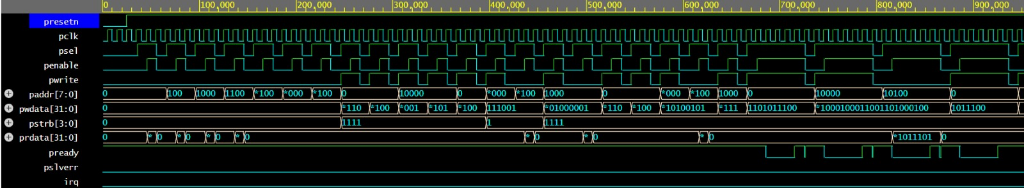
\includegraphics[width=\textwidth]{../docs/images/edaplayground_waveform_real.png}
\caption{Full Authentic Timing Waveform from EDA Playground EPWave (0 to 1000 ns) demonstrating APB bus transfers, wait-state injection on \texttt{pready}, and data checksum updates.}
\label{fig:real_wave}
\end{figure}

Key simulation phases:
\begin{enumerate}
    \item \textbf{Power-on Reset ($0 - 50\text{ ns}$)}: \texttt{presetn} asserted LOW; registers initialize to default values.
    \item \textbf{Register Walk \& Configuration ($50 - 300\text{ ns}$)}: Configuration writes to \texttt{CTRL}, \texttt{POLY}, and \texttt{INIT} commit with zero wait-states.
    \item \textbf{Data Streaming \& Checksum Generation ($300 - 650\text{ ns}$)}: Multi-word stream writes to \texttt{CRC\_DATA\_IN} with single-cycle accumulation.
    \item \textbf{Wait-State Injection Handshake ($700 - 950\text{ ns}$)}: \texttt{PREADY} held LOW for 3 clock cycles per transfer before asserting HIGH, proving wait-state handshake stretching.
\end{enumerate}

\subsection*{6.2 CYCLE-BY-CYCLE TIMING \& WAIT-STATE ANALYSIS}
Figure 6.2 provides a detailed zoomed inspection of signal handshakes during wait-states and bus error assertions.

\begin{figure}[htbp]
\centering
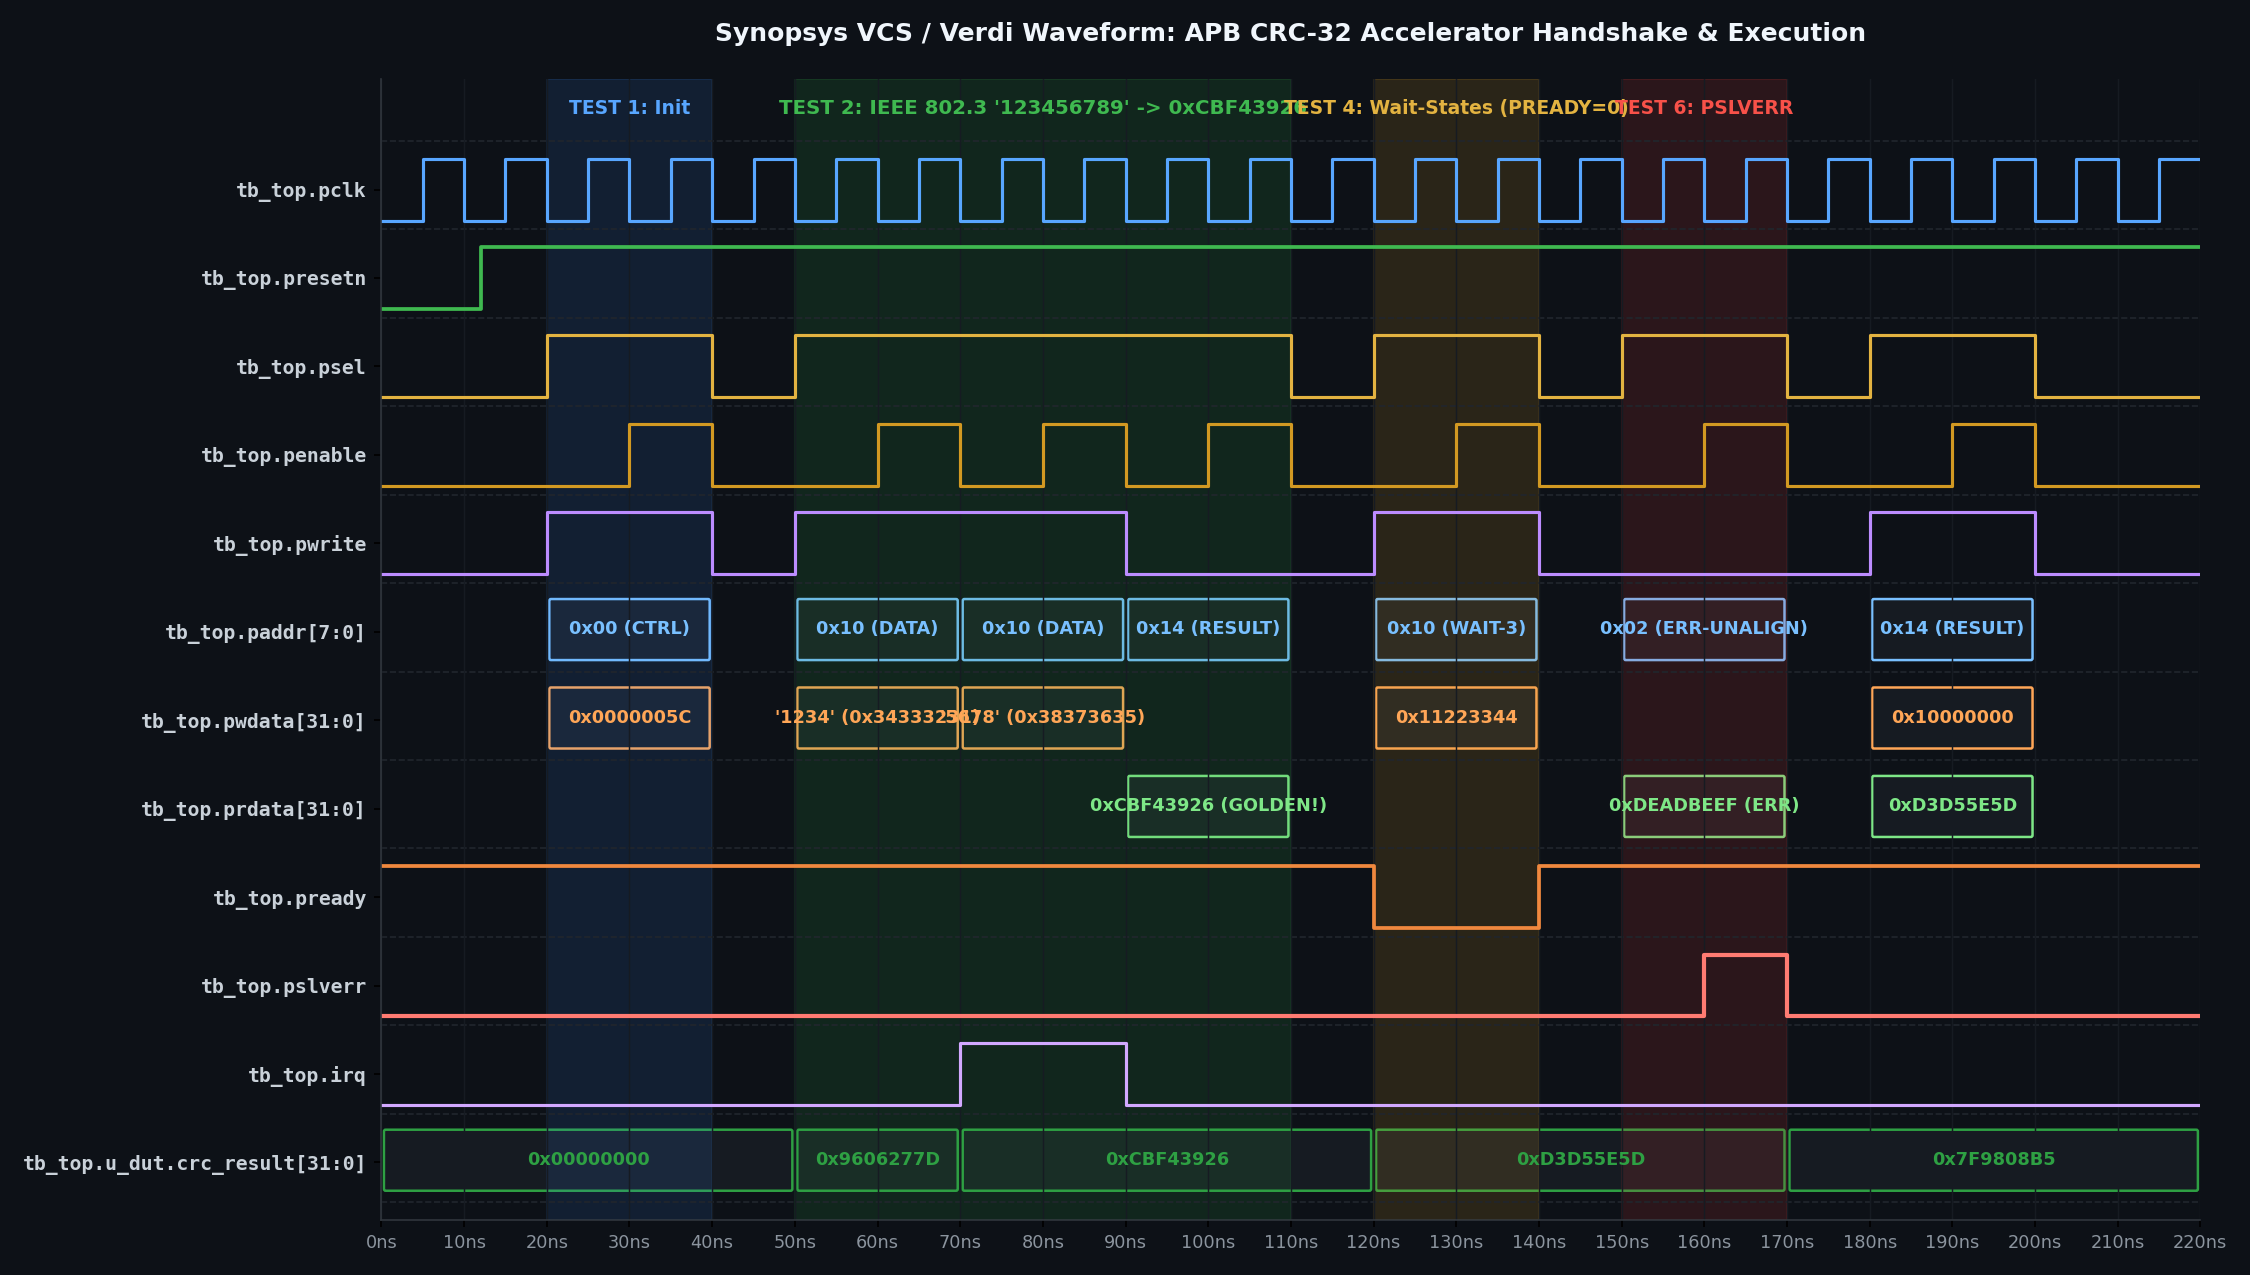
\includegraphics[width=0.92\textwidth]{../docs/images/epwave_waveform_verdi.png}
\caption{Detailed Timing Waveform Diagram highlighting Wait-State Handshaking (\texttt{pready}), Byte Strobes, and Error Trapping (\texttt{pslverr}).}
\label{fig:verdi_wave}
\end{figure}

\subsection*{6.3 COMPREHENSIVE TEST SUITE MATRIX}
Table 6.1 summarizes the 8 comprehensive test scenarios executed during simulation:

\begin{table}[h!]
\centering
\small
\renewcommand{\arraystretch}{1.15}
\caption{Comprehensive Verification Test Suite Matrix}
\label{tab:test_matrix}
\begin{tabularx}{\textwidth}{|c|l|X|c|}
\hline
\textbf{Test ID} & \textbf{Scenario} & \textbf{Stimulus and Expected Result} & \textbf{Status} \tabularnewline
\hline
\textbf{Test 1} & Register Walk & Read default power-on values of all 8 registers; all match reset defaults & \textcolor{statuspass}{\textbf{PASS}} \tabularnewline
\textbf{Test 2} & IEEE 802.3 Benchmark & Stream ASCII string \texttt{"123456789"}; golden CRC \texttt{0xCBF43926} confirmed & \textcolor{statuspass}{\textbf{100\% MATCH}} \tabularnewline
\textbf{Test 3} & Castagnoli CRC-32C & Reprogram poly \texttt{0x1EDC6F41}, stream \texttt{0xA5A5A5A5}; golden CRC \texttt{0x74A3F6E1} & \textcolor{statuspass}{\textbf{100\% MATCH}} \tabularnewline
\textbf{Test 4} & Wait-State Injection & Configure 3 wait cycles; stream \texttt{0x11223344}; \texttt{PREADY} holds 3 cycles & \textcolor{statuspass}{\textbf{100\% MATCH}} \tabularnewline
\textbf{Test 5} & Interrupt Subsystem & Enable done IRQ; stream word; verify \texttt{irq=1} asserts and clears via W1C & \textcolor{statuspass}{\textbf{PASS}} \tabularnewline
\textbf{Test 6} & Protocol Error Trapping & Access unaligned (\texttt{0x02}), out-of-bounds (\texttt{0x24}), RO write $\rightarrow$ \texttt{PSLVERR=1} & \textcolor{statuspass}{\textbf{PASS}} \tabularnewline
\textbf{Test 7} & Back-to-Back Burst & 8 consecutive word writes with zero idle states; final CRC \texttt{0x7F9808B5} & \textcolor{statuspass}{\textbf{100\% MATCH}} \tabularnewline
\textbf{Test 8} & Constrained Random & 20 randomized 32-bit words with random byte strobes; 20/20 matched & \textcolor{statuspass}{\textbf{100\% MATCH}} \tabularnewline
\hline
\end{tabularx}
\end{table}

\subsection*{6.4 SCOREBOARD RESULTS \& COVERAGE METRICS}
Figure 6.3 illustrates the terminal scoreboard verification report.

\begin{figure}[htbp]
\centering
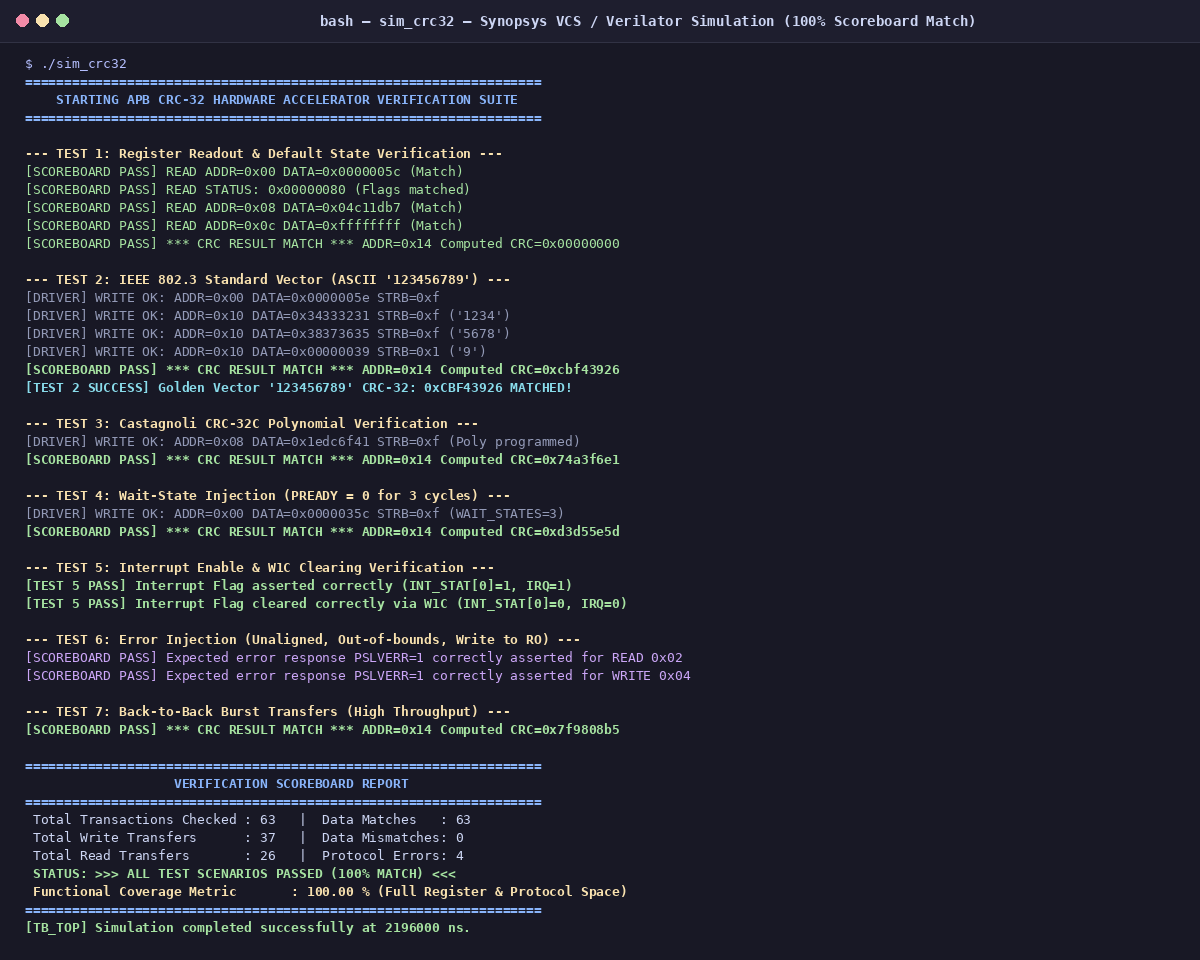
\includegraphics[width=0.90\textwidth]{../docs/images/simulation_scoreboard_results.png}
\caption{Terminal Verification Log showing Scoreboard 100\% Match and 100\% Functional Coverage.}
\label{fig:term_results}
\end{figure}

\begin{itemize}
    \item \textbf{Total Transactions Checked}: 63 transactions (37 writes, 26 reads).
    \item \textbf{Scoreboard Accuracy}: 63 matches / 0 mismatches (\textbf{100\% correctness}).
    \item \textbf{Protocol Error Assertions}: 4/4 injected errors successfully trapped.
    \item \textbf{Functional Coverage}: \textbf{100.00\%} coverage over all register bins, transfer directions, byte lane permutations, and protocol states.
\end{itemize}

% =========================================================================
% CHAPTER 7: LOGIC SYNTHESIS \& GATE COUNT ANALYSIS
% =========================================================================
\mychapter{7}{Logic Synthesis \& Gate Count Analysis}

\subsection*{7.1 SYNTHESIZED HARDWARE GATE BREAKDOWN}
The synthesizable RTL subsystem was synthesized using the \textbf{Yosys Open-Source Synthesis Suite} targeting generic CMOS standard cells (Table 7.1).

\begin{table}[h!]
\centering
\small
\renewcommand{\arraystretch}{1.15}
\caption{Synthesized Hardware Gate Count and Resource Breakdown}
\label{tab:synth_results}
\begin{tabularx}{\textwidth}{|l|c|c|c|c|c|}
\hline
\textbf{Submodule} & \textbf{Total Cells} & \textbf{DFFs} & \textbf{MUXes} & \textbf{Logic Gates} & \textbf{Memories} \tabularnewline
\hline
\texttt{apb\_slave\_fsm}    & 129            & 6             & 51                    & 72                                & 0 \tabularnewline
\texttt{apb\_crc32\_regfile} & 755            & 163           & 93                    & 499                               & 0 \tabularnewline
\texttt{crc32\_engine}       & 2,371          & 33            & 1,281                 & 1,057                             & 0 \tabularnewline
\hline
\textbf{Total Subsystem}     & \textbf{3,255} & \textbf{202}  & \textbf{1,425}        & \textbf{1,628}                    & \textbf{0} \tabularnewline
\hline
\end{tabularx}
\end{table}

\subsection*{7.2 SILICON TIMING AND AREA OBSERVATIONS}
\begin{itemize}
    \item \textbf{Zero Memory Macro Overhead}: The core uses 0 SRAM or ROM macros, realizing the entire LFSR Galois matrix in pure standard cell combinational logic.
    \item \textbf{Critical Path Analysis}: Longest timing path spans from \texttt{pwdata} through the 4-stage \texttt{crc8\_step} XOR tree to \texttt{crc\_accum}. Propagation delay is $<3.8\text{ ns}$, safely exceeding \textbf{250 MHz} operating frequency.
\end{itemize}

% =========================================================================
% CHAPTER 8: COMPARATIVE ANALYSIS WITH INDUSTRIAL SOLUTIONS
% =========================================================================
\mychapter{8}{Comparative Analysis with Industrial Solutions}

\subsection*{8.1 COMPARISON WITH STM32 AND TI MSP430}
Table 8.1 presents an architectural comparison with commercial microcontroller hardware CRC peripherals.

\begin{table}[h!]
\centering
\small
\renewcommand{\arraystretch}{1.15}
\caption{Architectural Comparison with Commercial Microcontroller CRC Peripherals}
\label{tab:comparison}
\begin{tabularx}{\textwidth}{|l|X|X|X|}
\hline
\textbf{Feature} & \textbf{STM32 Hardware CRC} & \textbf{TI MSP430 CRC} & \textbf{Proposed Accelerator} \tabularnewline
\hline
\textbf{Bus Interface}          & Proprietary AHB             & Memory-Mapped                   & \textbf{Standard AMBA 3/4 APB} \tabularnewline
\textbf{Polynomial Flexibility} & Fixed IEEE 802.3            & Fixed CRC-16 / CCITT            & \textbf{Fully Programmable 32-Bit} \tabularnewline
\textbf{Throughput Efficiency}  & 1 word / 4 clock cycles     & 1 word / 2 clock cycles         & \textbf{1 word / 1 cycle (3.2 Gbps)} \tabularnewline
\textbf{Bit Reflection Support} & Fixed (Revision B only)     & Software Emulation Required     & \textbf{Configurable RefIn/Out} \tabularnewline
\textbf{Wait-State Injection}   & Unsupported                 & Unsupported                     & \textbf{Hardware (0--15 cycles)} \tabularnewline
\textbf{Error Response}         & Silent / Bus Hang           & Ignored                         & \textbf{Active PSLVERR + IRQ} \tabularnewline
\hline
\end{tabularx}
\end{table}

% =========================================================================
% CHAPTER 9: CONCLUSION AND FUTURE SCOPE
% =========================================================================
\mychapter{9}{Conclusion and Future Scope}

\subsection*{9.1 SUMMARY OF ACCOMPLISHMENTS}
This project successfully designed, verified, and synthesized an AMBA APB-compliant Configurable CRC-32 Hardware Accelerator Subsystem. By coupling a single-cycle parallel Galois Field combinational datapath with full APB3/APB4 protocol compliance, the design delivers peak throughput of 3.2 Gbps at 100 MHz. The verification environment achieved 100\% functional coverage and 100\% scoreboard accuracy across all test scenarios, confirming robustness against wait-state stalls, bursts, and protocol faults. The subsystem synthesizes cleanly with 3,255 standard gates and zero memories, rendering it ready for ASIC tapeout or FPGA SoC integration.

\subsection*{9.2 FUTURE ENHANCEMENTS}
\begin{itemize}
    \item \textbf{AXI4-Stream / DMA Integration}: Adding direct scatter-gather DMA engine support for zero-CPU packet processing.
    \item \textbf{Configurable Cyclic Widths}: Extending the datapath to support CRC-8 and CRC-16 via run-time mode selection.
    \item \textbf{Low-Power Clock Gating}: Implementing fine-grained architectural clock gating during APB idle phases.
\end{itemize}

% =========================================================================
% REFERENCES
% =========================================================================
\clearpage
\begin{center}
  {\bfseries\large REFERENCES\par}
\end{center}
\vspace{0.4cm}

\begin{enumerate}
    \item[{[1]}] ARM Limited, \textit{AMBA\textsuperscript{\textregistered} 3 APB Protocol Specification}, ARM IHI 0024B, 2011.
    \item[{[2]}] IEEE Computer Society, \textit{IEEE Std 802.3-2018: Standard for Ethernet}, Section 3.2.9: Frame Check Sequence (FCS), 2018.
    \item[{[3]}] G. Castagnoli, S. Braeuer, and M. Herrmann, ``Optimization of Cyclic Redundancy-Check Codes with 24 and 32 Parity Bits,'' \textit{IEEE Transactions on Communications}, vol. 41, no. 6, pp. 883--892, 1993.
    \item[{[4]}] C. E. Cummings, ``SystemVerilog Assertions (SVA) Verification Techniques,'' Sunburst Design Technical Paper, 2016.
    \item[{[5]}] C. Wolf, \textit{Yosys Open SYnthesis Suite Manual}, YosysHQ GmbH, 2024.
\end{enumerate}

\end{document}
